\section{Weryfikacja rozwiązania}
\subsection{Przykład uruchomienia programu}
W celu skorzystania z programu agilemaster, należy stworzyć wspomniane wcześniej pliki z danymi użytkownika oraz danymi dostępowymi do api.
Następnie, wprowadzamy do programu wybrane parametry. Nazwa projektu musi zgadzać się z nazwą projektu stworzonego na instancji Jiry, podobnie jak nazwy statusów.
Kolejność podania statusów ma znaczenie, ponieważ bez dodatkowej konfiguracji nie jest możliwy inny sposób ustalenia ich naturalnej progresji.
\begin{lstlisting}[caption=Przykładowe użycie programu agilemaster]
PS C:\Users\Kuba\RustroverProjects\agilemaster> agilemaster `
>> --name kanban-test `
>> --author user.json `
>> --auth auth.json `
>> --start 01-02-2024 `
>> --end 31-03-2024 `
>> --issues 70 `
>> --statuses "BACKLOG" "SELECTED FOR DEVELOPMENT" "IN PROGRESS" "DONE"
\end{lstlisting}

W efekcie takiego wywołania tworzony jest plik \texttt{kanban-test.json} (nazwa wygenerowana na podstawie podanej nazwy projektu).
Należy stworzyć pusty projekt typu Kanban, a następnie na swojej instancji Jiry w ustawieniach wybrać kategorię "System", a następnie zakładkę "External System Import".
Należy zwrócić uwagę że w przypadku wyboru konfiguracji "Team-managed" i "Company-managed" w projekcie domyślnie mamy dostępne inne statusy.
Statusy w projekcie można dowolnie dostosować, pamiętając jednak aby poprawnie podać je przy użyciu programu agilemaster.
\begin{figure}[H]
    \centering
    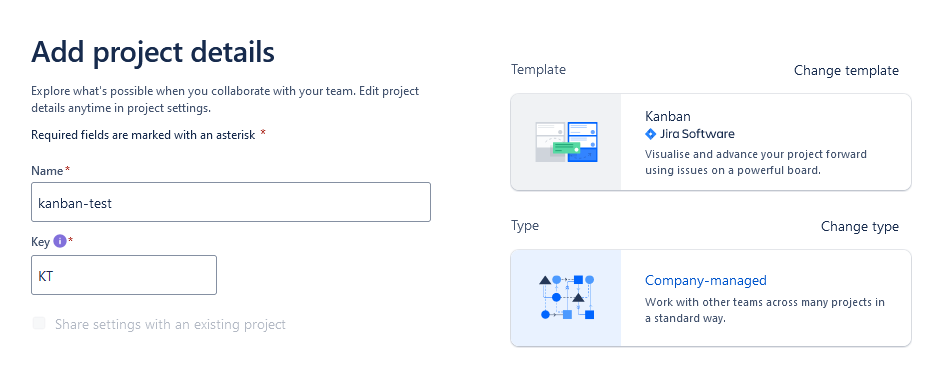
\includegraphics[width=15cm,keepaspectratio]{rysunki/jira-create-project.png}
    \caption{Tworzenie projektu Kanban w konfiguracji Company-managed}
\end{figure}

\begin{figure}[H]
    \centering
    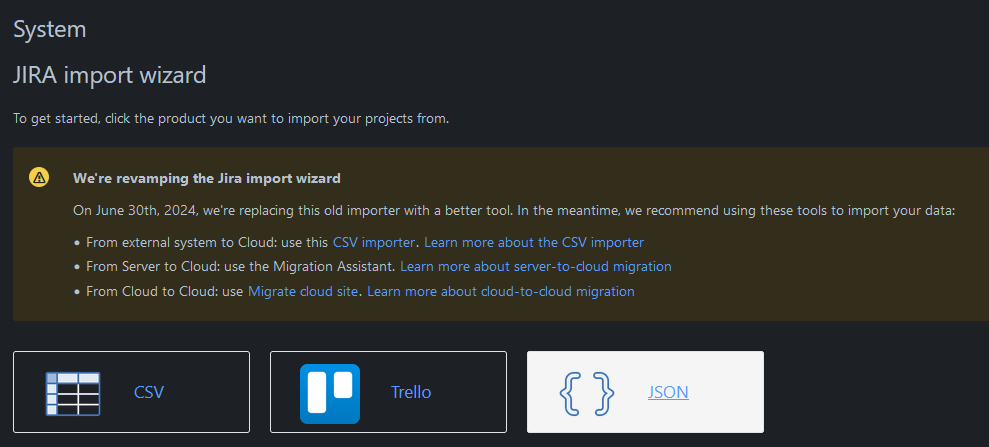
\includegraphics[width=15cm,keepaspectratio]{rysunki/jira-import-wizard.png}
    \caption{Narzędzie do importu danych na Jirę}
\end{figure}

Po pomyślnym zakończeniu importu danych, wszystkie zadania możemy zaobserwować w projekcie.
\begin{figure}[H]
    \centering
    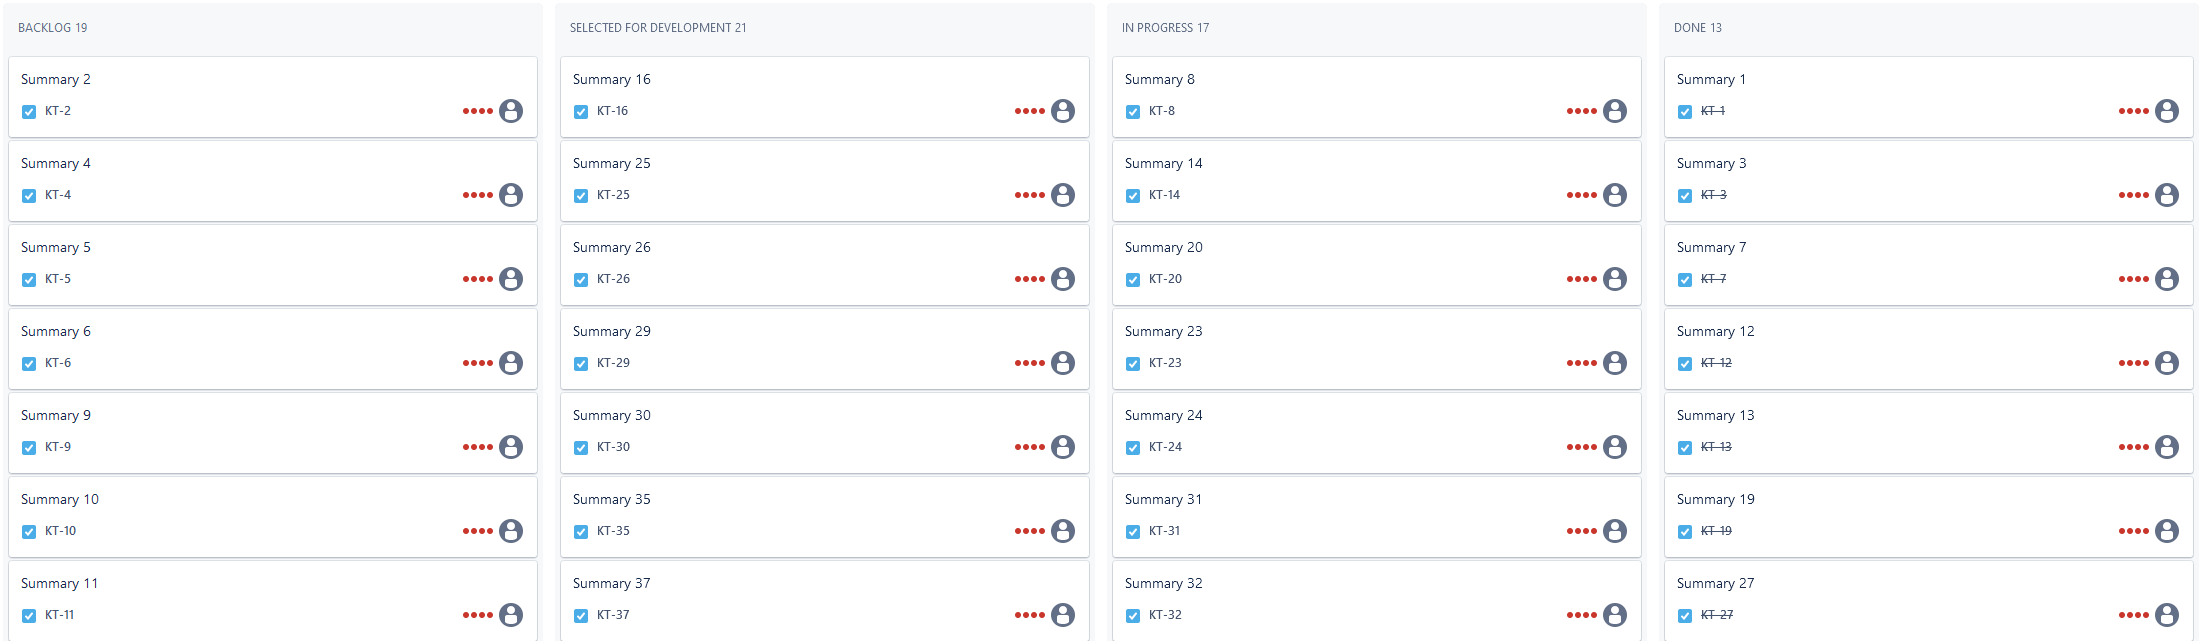
\includegraphics[width=15cm,keepaspectratio]{rysunki/jira-board.png}
    \caption{Fragement tablicy wypełnionej zaimportowanymi zadaniami}
\end{figure}

Przy inspekcji zakładki "History" w zadaniu możemy zaobserwować poprawną chronologię w zmianach statusów.
\begin{figure}[H]
    \centering
    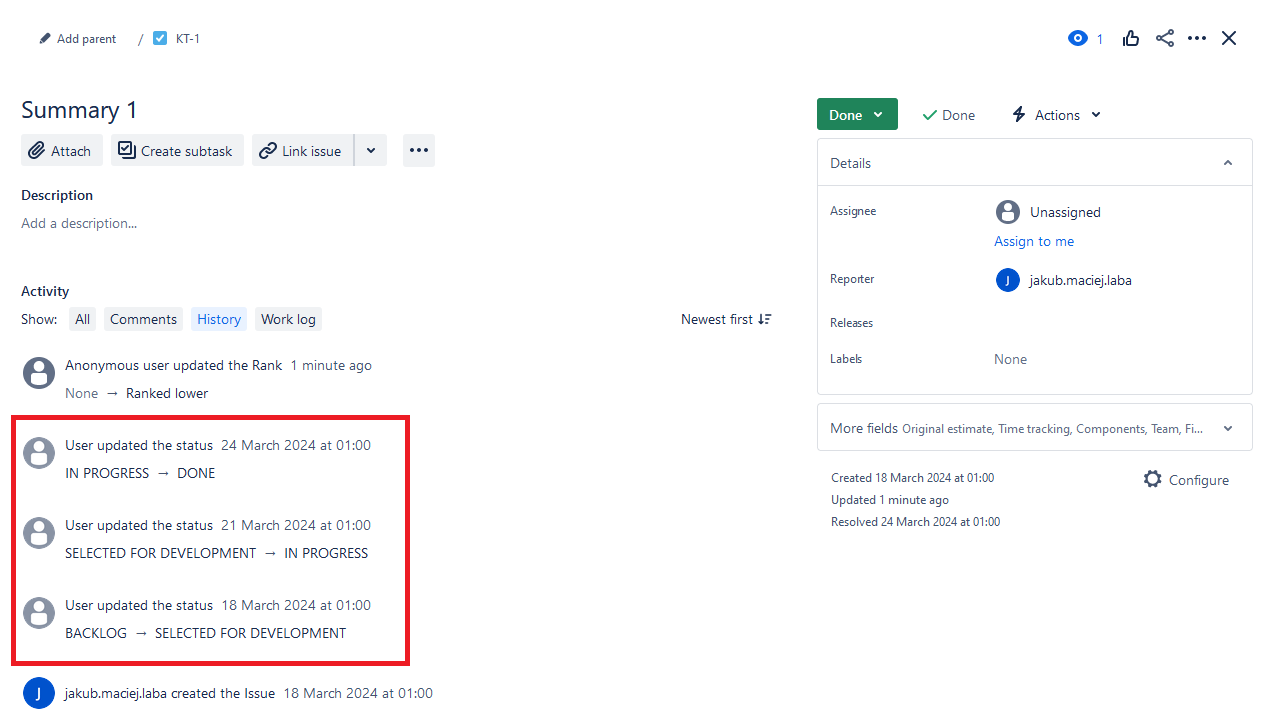
\includegraphics[width=15cm,keepaspectratio]{rysunki/jira-issue-history.png}
    \caption{Historia przykładowego zaimportowanego zadania}
\end{figure}

\subsection{Przykład analizy metryk}
Z uwagi na fakt, że zaimplementowanie integracji z wbudowanymi narzędziami analitycznymi nie było możliwe, niestety nie można przeprowadzić analizy metryk bezpośrednio na Jirze. Nadal można jednak łatwo wydobyć potrzebne
dane za pomocą JQL, a następnie obliczyć je w arkuszu kalkulacyjnym lub narzędziu do analizy biznesowej.

Ten podrozdział prezentuje przykładowe zapytania JQL, które można zastosować do wydobycia danych potrzebnych do analizy metryk.

\subsubsection*{Wiek pracy w toku}
W celu obliczenia wieku pracy w toku dla konkretnego zadania, można wydobyć je prostym zapytaniem o klucz: \lstinline{key = "KT-3"}.
Następnie należy obliczyć ilość dni pomiędzy obecną datą, a datą utworzenia zadania.
Na podobnej zasadzie można obliczyć średni wiek pracy w toku dla większej ilości zadań dla celów monitorowania produktywności, aby szybko identyfikować blokujące się zadania gdy zaczynają znacznie przekraczać średnią wartość tej metryki.

\subsubsection*{Przepustowość}
Przepustowość można otrzymać licząc ilość wyników zwróconych przez zapytanie JQL, filtrujące zadania po przejściu do wybranego statusu oznaczającego zakończenie zadania, oraz w wybranym przedziale czasowym.
\begin{lstlisting}[caption=Zapytanie JQL pozwalające obliczyć przepustowość w przeciągu ostatniego tygodnia]
status CHANGED TO "Done" DURING (-7d, now())
\end{lstlisting}

\subsubsection*{Efektywność przepływu}
Do obliczenia efektywności przepływu potrzeba zidentyfikować które statusy były aktywne, a które pasywne.

W rozpatrywanym tutaj przypadku testowym, jedynym aktywny statusem był "In Progress", należy więc znaleźć wszystkie zadania które znajdowały się w tym statusie.
\begin{lstlisting}[caption=Zapytanie JQL pozwalające obliczyć efektywność przepływu]
status WAS "In Progress"
\end{lstlisting}

W otrzymanych wynikach wyszukiwania za pomocą wybranego narzędzia należy obliczyć całkowity czas znajdowania się w statusach aktywnych i pasywnych, oraz obliczyć proporcję jednego do drugiego.

\subsubsection*{Czas realizacji}
Do obliczenia czasu realizacji potrzeba zdefiniować który status jest punktem realizacji, a który punktem dostarczenia.

W rozpatrywanym tutaj przypadku testowym, punktem zobowiązania był status "Selected for Development", natomiast punktem dostarczenia status "Done".
\begin{lstlisting}[caption=Zapytanie JQL pozwalające obliczyć czas dostarczenia w przeciągu ostatniego tygodnia]
status WAS "Selected for Development" DURING (-7d, now())
AND status CHANGED TO "Done" DURING(-7d, now())
\end{lstlisting}

Następnie w wybranym narzędziu należy obliczyć okres pomiędzy datami znalezienia się zadania w tych dwóch statusach.
Na podobnej zasadzie można obliczyć średni czas realizacji dla większej ilości zadań w celu zdobycia danych do estymacji jakie zobowiązania można podjąć wobec klienta.
